\documentclass{beamer}
\usepackage[utf8]{inputenc}
  
\usetheme{Madrid}
\usecolortheme{default}
\usepackage{amsmath,amssymb,amsfonts,amsthm}
\usepackage{txfonts}
\usepackage{tkz-euclide}
\usepackage{listings}
\usepackage{adjustbox}
\usepackage{array}
\usepackage{tabularx}
\usepackage{gvv}
\usepackage{lmodern}
\usepackage{circuitikz}
\usepackage{tikz}
\usepackage{graphicx}
\usepackage[T1]{fontenc}
\UseRawInputEncoding

\setbeamertemplate{page number in head/foot}[totalframenumber]

\usepackage{tcolorbox}
\tcbuselibrary{minted,breakable,xparse,skins}



\definecolor{bg}{gray}{0.95}
\DeclareTCBListing{mintedbox}{O{}m!O{}}{%
  breakable=true,
  listing engine=minted,
  listing only,
  minted language=#2,
  minted style=default,
  minted options={%
    linenos,
    gobble=0,
    breaklines=true,
    breakafter=,,
    fontsize=\small,
    numbersep=8pt,
    #1},
  boxsep=0pt,
  left skip=0pt,
  right skip=0pt,
  left=25pt,
  right=0pt,
  top=3pt,
  bottom=3pt,
  arc=5pt,
  leftrule=0pt,
  rightrule=0pt,
  bottomrule=2pt,
  toprule=2pt,
  colback=bg,
  colframe=orange!70,
  enhanced,
  overlay={%
    \begin{tcbclipinterior}
    \fill[orange!20!white] (frame.south west) rectangle ([xshift=20pt]frame.north west);
    \end{tcbclipinterior}},
  #3,
}
\lstset{
    language=C,
    basicstyle=\ttfamily\small,
    keywordstyle=\color{blue},
    stringstyle=\color{orange},
    commentstyle=\color{green!60!black},
    numbers=left,
    numberstyle=\tiny\color{gray},
    breaklines=true,
    showstringspaces=false,
}



\title 
{MatGeo Assignment 9.2.41}

\author
{AI25BTECH11007}
\begin{document}

\frame{\titlepage}
\begin{frame}{Question}
     Find the area of the region bounded by the curves $y^2$ = 9x, y = 3x.
\end{frame}

\begin{frame}{Solution}
    \begin{align}
  \text{Given curves: } 
  & y^2 = 9x, \quad y = 3x
\end{align}
The conic can be written as
\begin{align}
g(\vec{x}) = \vec{x}^T\vec{V}\vec{x} + 2\vec{u}^T\vec{x} + f = 0
\end{align}
where
\begin{align}
\vec{V} = \myvec{0 & 0 \\ 0 & 1}, \quad
\vec{u} = \myvec{-\tfrac{9}{2} \\ 0}, \quad
f = 0
\end{align}

The equation of the line is
\begin{align}
\vec{x} = \vec{h} + \kappa \vec{m}
\end{align}
where
\begin{align}
\vec{h} = \myvec{0 \\ 0}, \quad 
\vec{m} = \myvec{1 \\ 3}
\end{align}

Substituting in $g(\vec{x}) = 0$:
\end{frame}

\begin{frame}
    \begin{align}
(\vec{h} + \kappa\vec{m})^T\vec{V}(\vec{h} + \kappa\vec{m})
+ 2\vec{u}^T(\vec{h} + \kappa\vec{m}) + f = 0
\end{align}

Expanding,
\begin{align}
\kappa^2 (\vec{m}^T\vec{V}\vec{m}) + 2\kappa(\vec{m}^T(\vec{V}\vec{h} + \vec{u})) + (\vec{h}^T\vec{V}\vec{h} + 2\vec{u}^T\vec{h} + f) = 0
\end{align}

Substituting the known values,
\begin{align}
9\kappa^2 - 9\kappa = 0
\end{align}
\[
\kappa_1 = 0, \quad \kappa_2 = 1
\]

\noindent
Finally, intersecting points are
\begin{align}
\vec{x}_1 &= \myvec{0 \\ 0} + 0\myvec{1 \\ 3} = \myvec{0 \\ 0} \\[2mm]
\vec{x}_2 &= \myvec{0 \\ 0} + 1\myvec{1 \\ 3} = \myvec{1 \\ 3}
\end{align}
\end{frame}

 \begin{frame}
     
\noindent
Thus, the points of intersection are 
\[
A = \myvec{0 \\ 0}, \quad B = \myvec{1 \\ 3}
\] 
 
Hence, the required area is
\begin{align}
A &= \int_{0}^{1} (3\sqrt{x} - 3x)\,dx \\[2mm]
\end{align}
\[
\boxed{A = \tfrac{1}{2} \text{ square units}}
\]
 \end{frame}

\begin{frame}{Plot}
    \begin{figure}
    \centering
    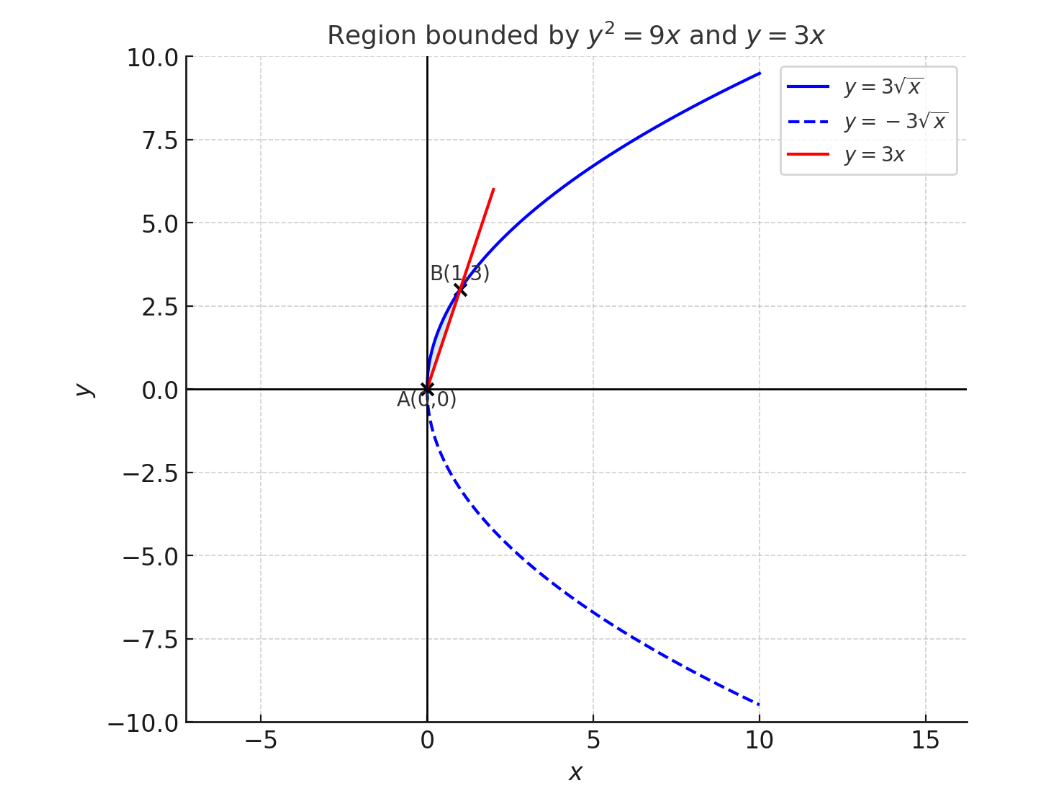
\includegraphics[width=0.85\linewidth]{figs/image.png}
    \caption{Image}
    \label{fig:placeholder}
\end{figure}
\end{frame}

\begin{frame}[fragile]{C code}
    \begin{lstlisting}
        #include <stdio.h>
#include <math.h>

// Function for the parabola y = 3*sqrt(x)
double parabola(double x) {
    return 3 * sqrt(x);
}

// Function for the line y = 3*x
double line(double x) {
    return 3 * x;
}

// Function to compute area using trapezoidal rule
double area_between_curves(double a, double b, int n) {
    double h = (b - a) / n;
    double area = 0.0;
    for(int i = 0; i <= n; i++) {
        double x = a + i*h;
    \end{lstlisting}
\end{frame}

\begin{frame}[fragile]{C code}
    \begin{lstlisting}
        double y_diff = parabola(x) - line(x);
        if(i == 0 || i == n)
            area += y_diff / 2.0;
        else
            area += y_diff;
    }
    area *= h;
    return area;
}

int main() {
    double a = 0.0, b = 1.0; // limits of integration (intersection points)
    int n = 1000; // number of subintervals for numerical integration

    double area = area_between_curves(a, b, n);
    printf("Area enclosed between y^2 = 9x and y = 3x: %.6f square units\n", area);
    \end{lstlisting}
\end{frame}

\begin{frame}[fragile]{C code}
    \begin{lstlisting}
         // Direct symbolic calculation
    double symbolic_area = 3.0*(2.0/3.0 - 0.5);
    printf("Area calculated symbolically: %.6f square units\n", symbolic_area);
    return 0;
}
    \end{lstlisting}
\end{frame}

\begin{frame}[fragile]{Python code}
    \begin{lstlisting}
        import numpy as np
import matplotlib.pyplot as plt

# Define x range for the parabola (both branches)
x = np.linspace(0, 10, 400)
y_upper = 3 * np.sqrt(x)
y_lower = -3 * np.sqrt(x)

# Line y = 3x
x_line = np.linspace(0, 2, 200)
y_line = 3 * x_line

# Plot setup
plt.figure(figsize=(7,6))
plt.plot(x, y_upper, 'b', label=r'$y = 3\sqrt{x}$')
plt.plot(x, y_lower, 'b', linestyle='--', label=r'$y = -3\sqrt{x}$')
plt.plot(x_line, y_line, 'r', label=r'$y = 3x$')
    \end{lstlisting}
\end{frame}

\begin{frame}[fragile]{Python code}
    \begin{lstlisting}
x_fill = np.linspace(0, 1, 200)
plt.fill_between(x_fill, 3*x_fill, 3*np.sqrt(x_fill), color='lightblue', alpha=0.5)
# Mark intersection points
plt.scatter([0,1], [0,3], color='black')
plt.text(0, -0.5, 'A(0,0)', ha='center', fontsize=10)
plt.text(1, 3.3, 'B(1,3)', ha='center', fontsize=10)
plt.axhline(0, color='k', linewidth=1)
plt.axvline(0, color='k', linewidth=1)
plt.title(r'Region bounded by $y^2 = 9x$ and $y = 3x$', fontsize=13)
plt.xlabel(r'$x$')
plt.ylabel(r'$y$')
plt.legend(loc='upper right')
plt.grid(True, linestyle='--', alpha=0.6)
plt.axis('equal')
plt.xlim(-1, 10)
plt.ylim(-10, 10)
plt.show()
    \end{lstlisting}
\end{frame}

\end{document}